% ============================================================================
%  LectureAssist -- Senior Design Project (499) poster
%
%  Build:  lualatex poster.tex        (luainputenc requires LuaLaTeX)
%
%  DATA PROVENANCE -- read before editing any number in this file.
%  Every figure on this poster comes from the ONE evaluation run that actually
%  completed: the native-metrics run, n=200 MCQ per pipeline, reported in
%  Book/4.results.tex Tables tab:native-overall and tab:native-difficulty.
%
%  NOTE ON COLUMN ORDER: Book/4.results.tex Table tab:native-overall has its two
%  data columns swapped relative to its headers. Proof: semantic grounding and
%  independent-answer match are plain means, so the per-difficulty table must
%  pool exactly. The rows labelled "Agentic" there pool to 0.5567 grounding and
%  0.9403 match -- the values printed under the book's "Non-Agentic" heading.
%  The book's own prose (4.results.tex:596-601) and its tab:loo / tab:merge
%  control row (agentic = 0.385 / 0.557 / 0.612 / 0.940) agree with the pooling,
%  not with the table headers. THIS POSTER USES THE CORRECTED ASSIGNMENT.
%
%  Deliberately NOT on this poster:
%    - EQGBench figures (Book tab:eqg-compare). No completed run backs them; the
%      only artifact is eval_out_eqgbench_OLD-unfaithful-protocol/, a repudiated
%      protocol whose log ends in continuous 429 judge failures and which
%      contains 1 successfully-judged agentic row and zero non-agentic rows.
%    - ReQUESTA figures (tab:req-compare). Mostly pending cells upstream.
%    - Leave-one-out and agent-merging figures (tab:loo, tab:merge). Chapter 4
%      states at :118-127 that these configurations are "built, unrun" / "not yet
%      implemented". They are shown here as PENDING, which is what that text
%      promises.
% ============================================================================

\documentclass[final]{beamer}

\usepackage[T1]{fontenc}
\usepackage[utf8]{luainputenc}
\usepackage{lmodern}
\usepackage[size=a0, orientation=landscape, scale=1.1]{beamerposter}
\usetheme{gemini}
\usecolortheme{gemini}
\usepackage{graphicx}
\usepackage{booktabs}
\usepackage{tikz}
\usepackage{amsmath, amssymb}
\usepackage{pgfplots}
\pgfplotsset{compat=1.14}
\usepackage{anyfontsize}
\usetikzlibrary{arrows.meta, positioning, shapes.geometric, calc, fit, backgrounds}

\newlength{\sepwidth}
\newlength{\colwidth}
\setlength{\sepwidth}{0.025\paperwidth}
\setlength{\colwidth}{0.3\paperwidth}

\newcommand{\separatorcolumn}{\begin{column}{\sepwidth}\end{column}}

\definecolor{LAindigo}{HTML}{6366F1}
\definecolor{LAviolet}{HTML}{A78BFA}
\definecolor{LAcyan}{HTML}{38BDF8}
\definecolor{LAgreen}{HTML}{34D399}
\definecolor{LAamber}{HTML}{FBBF24}
\definecolor{LAred}{HTML}{F87171}
\definecolor{LAink}{HTML}{2B2C45}
\definecolor{LAmist}{HTML}{EEF0FD}
\definecolor{LAslate}{HTML}{64748B}

\tikzset{
  labox/.style={rectangle, rounded corners=8pt, draw=LAindigo, line width=1.2pt,
    fill=white, text=LAink, align=center, inner sep=7pt, minimum height=1.5cm,
    font=\bfseries},
  lain/.style={labox, draw=LAcyan, fill=LAcyan!10},
  laproc/.style={labox, draw=LAviolet, fill=LAviolet!8},
  lallm/.style={labox, draw=LAamber, fill=LAamber!15},
  laout/.style={labox, draw=LAgreen, fill=LAgreen!12},
  laval/.style={labox, draw=LAred, fill=LAred!8},
  laarr/.style={-{Stealth[length=5mm,width=4mm]}, line width=1.6pt, draw=LAindigo},
  laarrg/.style={-{Stealth[length=5mm,width=4mm]}, line width=1.6pt, draw=LAgreen},
  laloop/.style={-{Stealth[length=5mm,width=4mm]}, line width=1.4pt, draw=LAred},
  lalbl/.style={font=\small\itshape, text=LAink, fill=white, inner sep=2pt},
}

% Marks the pipeline that wins a row. Used ONLY where the measurement supports it.
\newcommand{\win}[1]{\textbf{\textcolor{LAgreen}{#1}}}
\newcommand{\pend}{\textcolor{LAslate}{\emph{pending}}}

\title{LectureAssist: An Agentic, Multimodal AI Assistant that Turns Lectures into Adaptive Study Material}

\author{%
  \begin{tabular}{c@{\hspace{4cm}}c@{\hspace{4cm}}c}
    Iftikhar Ahmed & Salman Shafi & Jarinah Tasnim \\[2pt]
    {\normalsize\texttt{iftikhar.ahmed@northsouth.edu}} &
    {\normalsize\texttt{salman.shafi@northsouth.edu}} &
    {\normalsize\texttt{jarinah.tasnim@northsouth.edu}} \\
  \end{tabular}
}

\institute[NSU]{Dept.\ of Electrical and Computer Engineering, North South University \;\textbullet\; Senior Design Project (499) \;\textbullet\; Supervisor: Dr.\ Adnan Areefen}

\IfFileExists{uni.png}{\logoleft{
\includegraphics[height=8.5cm]{uni.png}}}{}

\begin{document}

\begin{frame}[t]
\begin{columns}[t]
\separatorcolumn

% ══════════════════════════ COLUMN 1 ══════════════════════════
\begin{column}{\colwidth}

  \begin{block}{Problem \& Goal}

    Recorded lectures pack speech, slides and board work into one video, and that
    content stays \textbf{locked and unsearchable}. Students re-watch hours of
    footage to find a single concept and have no fast way to self-test on what
    the lecturer actually emphasised.

    \begin{itemize}
      \item Lecture knowledge lives in \textbf{video, speech and board writing},
        rarely as clean text.
      \item Generic quiz tools \textbf{hallucinate} off-topic, ungrounded questions.
      \item One-size-fits-all difficulty ignores \textbf{each student's weak spots}.
    \end{itemize}

    \textbf{Goal.} A system that \emph{reads the board and hears the lecture}, and
    produces \emph{grounded, validated, adaptive} study material entirely on a
    free Colab T4 at \textbf{zero API cost}.

  \end{block}

  \begin{block}{System Architecture}

    A lecture video or document is extracted, indexed, and handed to an
    orchestrator that supervises specialist agents. Independent agents run
    concurrently; any agent crash is caught and logged so the pipeline
    \textbf{degrades gracefully} rather than failing outright.

    \begin{figure}
      \centering
      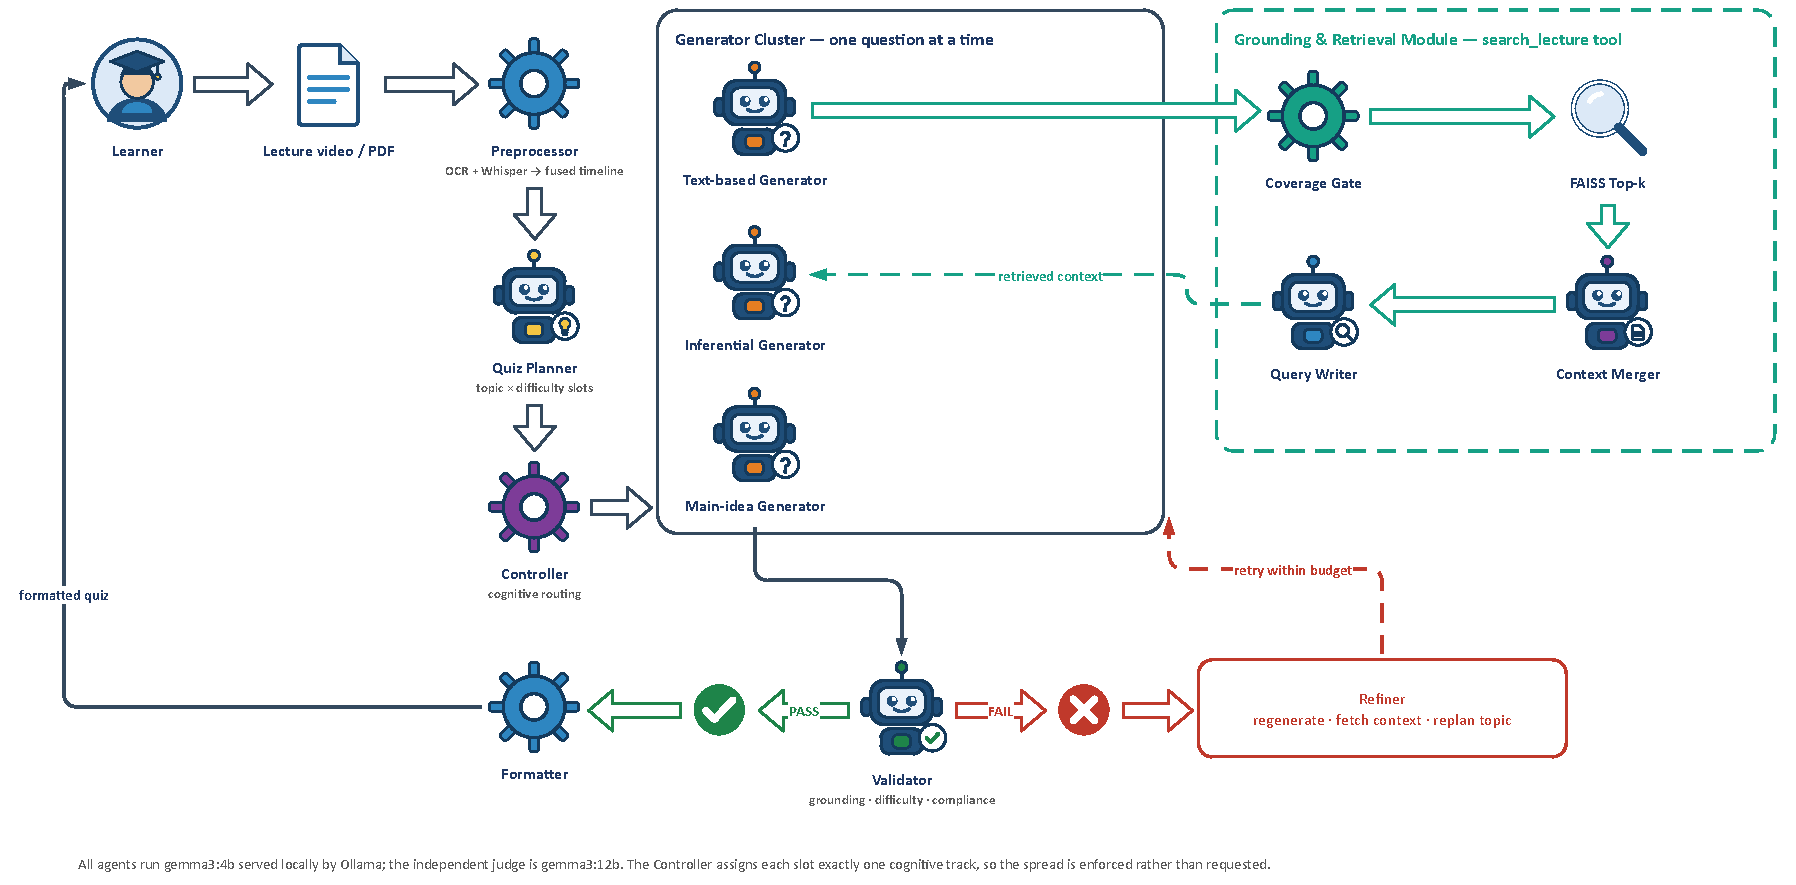
\includegraphics[width=\linewidth]{Book/lectureassist-architecture-illustrated.pdf}
      \caption{LectureAssist system architecture. Multimodal extraction feeds a
      grounded knowledge base; the orchestrator coordinates the specialist agents
      that produce every study artifact.}
    \end{figure}

  \end{block}

  \begin{block}{Stack}

    \begin{itemize}
      \item \textbf{Vision / OCR.} EasyOCR, frames sampled ${\sim}5$\,s apart and
        classified (slide / blackboard / whiteboard / scene) with per-class
        preprocessing --- CLAHE, sharpening, Otsu, chalk inversion.
      \item \textbf{Speech.} Faster-Whisper, GPU \texttt{float16} with CPU
        \texttt{int8} fallback, per-segment timestamps.
      \item \textbf{Retrieval.} Sentence-Transformers (\texttt{MiniLM}) embeddings
        in a \textbf{FAISS} cosine index; every artifact retrieves top-$k$ chunks
        before generation.
      \item \textbf{Models.} Generator \texttt{gemma3:4b} (pinned), judge and
        answer-generation \texttt{gemma3:12b}, served locally by Ollama.
      \item \textbf{Serving.} Flask on Colab $\rightarrow$ ngrok $\rightarrow$
        single-page browser UI.
    \end{itemize}

  \end{block}

\end{column}

\separatorcolumn

% ══════════════════════════ COLUMN 2 ══════════════════════════
\begin{column}{\colwidth}

  \begin{block}{The Agentic Loop}

    Questions are built \textbf{one at a time} and must \emph{pass validation}
    before the next slot begins. On failure the validator selects a remediation
    --- regenerate, fetch more context, or replan the topic. When the retry budget
    is exhausted the best attempt is kept and \textbf{marked as an override};
    a failed question is never silently relabelled as a pass.

    \begin{figure}
      \centering
      \begin{tikzpicture}[node distance=1.6cm and 1.6cm]
        \node[laproc, text width=8cm] (plan){\textbf{Planner}\\{\normalfont\small topics, mix}};
        \node[lallm, right=of plan, text width=8cm] (gen){\textbf{Generator}\\{\normalfont\small ONE question}};
        \node[laval, right=of gen, text width=9cm] (val){\textbf{Validator}\\{\normalfont\small grounded, difficulty, unique}};
        \node[lallm, below=1.9cm of gen, text width=8cm] (refine){\textbf{Refiner}\\{\normalfont\small targeted fix}};
        \node[laout, below=1.9cm of val, text width=8cm] (pass){\textbf{Accept}\\{\normalfont\small next slot}};
        \draw[laarr](plan)--(gen);
        \draw[laarr](gen)--(val);
        \draw[laarrg](val)--(pass) node[lalbl, midway, right]{PASS};
        \draw[laloop](val)--(refine) node[lalbl, midway, above]{FAIL};
        \draw[laloop](refine)--(gen) node[lalbl, midway, left]{retry $\le 3$};
      \end{tikzpicture}
      \caption{Plan $\rightarrow$ Generate $\rightarrow$ Validate $\rightarrow$
      Retry, budget-capped at three attempts per slot.}
    \end{figure}

  \end{block}

  \begin{block}{How We Evaluated It}

    Generation and measurement are kept \textbf{strictly separate}: the Colab run
    only emits questions, and judging happens offline on the exported artifact.

    \begin{itemize}
      \item \textbf{Source.} \emph{Limits} chapter of OpenStax \emph{Calculus,
        Vol.~1} (${\approx}112$k characters), ingested through the standard
        document pipeline and also supplied to the judge as ground truth.
      \item \textbf{Scale.} $n{=}200$ MCQ per pipeline, split across three target
        difficulties (easy $68$, medium $66$, hard $66$).
      \item \textbf{Fairness.} Both pipelines read the document through an
        identical sliding window with a uniform batch size, so neither sees more
        or different content --- any difference reflects \textbf{prompting
        strategy alone}.
      \item \textbf{Judge.} \texttt{gemma3:12b}, scoring questions written by the
        \texttt{gemma3:4b} generator.
    \end{itemize}

  \end{block}

  \begin{block}{Results by Difficulty}

    \begin{table}
      \centering
      \small
      \setlength{\tabcolsep}{5pt}
      \begin{tabular}{llccccc}
        \toprule
        \textbf{Diff.} & \textbf{Pipeline} & \textbf{$n$} &
        \textbf{Dup.}$\downarrow$ & \textbf{Ground.} &
        \textbf{Eff.\ acc.} & \textbf{Match} \\
        \midrule
        Easy   & Agentic     & 68 & 0.353 & 0.562 & 0.647 & 0.971 \\
               & Non-agentic & 68 & \win{0.324} & \win{0.642} & \win{0.676} & 0.971 \\
        \midrule
        Medium & Agentic     & 66 & 0.379 & 0.595 & 0.612 & 0.879 \\
               & Non-agentic & 66 & \win{0.227} & \win{0.614} & \win{0.773} & \win{0.955} \\
        \midrule
        Hard   & Agentic     & 66 & 0.288 & 0.513 & 0.712 & 0.970 \\
               & Non-agentic & 66 & \win{0.182} & \win{0.616} & \win{0.818} & \win{0.985} \\
        \bottomrule
      \end{tabular}
      \caption{The pattern is consistent at every difficulty level: the baseline
      leads on duplicate rate, grounding and effective acceptance throughout.}
    \end{table}

  \end{block}

  \begin{block}{Status \& Next Steps}

    \begin{table}
      \centering
      \small
      \begin{tabular}{ll}
        \toprule
        \textbf{Configuration} & \textbf{Status} \\
        \midrule
        \texttt{agentic}, \texttt{nonagentic} & scored, $n{=}200$ each \\
        \texttt{cot}, \texttt{pot}            & implemented, not judged \\
        \texttt{merge\_vr}, \texttt{merge\_pg} & built, \pend \\
        5 leave-one-agent-out configs         & specified, \pend \\
        EQGBench / ReQUESTA protocols         & harnesses built, \pend \\
        \bottomrule
      \end{tabular}
      \caption{No number is claimed for a run that has not completed. Next up are
      the leave-one-out ablations, which test the duplication hypothesis.}
    \end{table}

  \end{block}

\end{column}

\separatorcolumn

% ══════════════════════════ COLUMN 3 ══════════════════════════
\begin{column}{\colwidth}

  \begin{block}{Headline Results}

    \begin{table}
      \centering
      \small
      \begin{tabular}{lccc}
        \toprule
        \textbf{Metric} & \textbf{Scale} & \textbf{Agentic} & \textbf{Non-agentic} \\
        \midrule
        \multicolumn{4}{l}{\emph{Judged quality --- all four saturate}} \\
        Overall quality            & $1$--$5$ & 4.86  & \win{4.93} \\
        Correctness                & $1$--$5$ & 4.98  & \win{5.00} \\
        Clarity                    & $1$--$5$ & 4.92  & \win{4.97} \\
        Difficulty match           & $1$--$5$ & 4.36  & \win{4.39} \\
        \midrule
        \multicolumn{4}{l}{\emph{Automated --- these actually discriminate}} \\
        Duplicate rate $\downarrow$        & $0$--$1$ & 0.385 & \win{0.280} \\
        Semantic grounding                 & $0$--$1$ & 0.557 & \win{0.624} \\
        Effective acceptance               & $0$--$1$ & 0.612 & \win{0.720} \\
        Independent answer match           & $0$--$1$ & 0.940 & \win{0.970} \\
        Inter-question similarity $\downarrow$ & $0$--$1$ & 0.932 & \win{0.894} \\
        \midrule
        Acceptance rate            & $0$--$1$ & 0.995 & \win{1.000} \\
        Judge-verified correctness & $0$--$1$ & 0.995 & 0.995 \\
        \bottomrule
      \end{tabular}
      \caption{Native metrics, $n{=}200$ per pipeline. Green marks the better
      value; arrows mark rows where lower is better.}
    \end{table}

    \begin{figure}
      \centering
      \begin{tikzpicture}
        \begin{axis}[
          width=0.95\colwidth, height=13cm,
          ybar, bar width=1.5cm,
          ymin=0, ymax=0.85,
          enlarge x limits=0.22,
          symbolic x coords={Duplicate,Grounding,Eff. accept},
          xtick=data,
          ylabel={score},
          legend style={at={(0.5,1.06)}, anchor=south, legend columns=2, draw=none,
            column sep=1.2cm, /tikz/every even column/.append style={column sep=1.2cm}},
          nodes near coords, nodes near coords style={font=\small},
          every node near coord/.append style={/pgf/number format/fixed,
            /pgf/number format/precision=3, /pgf/number format/fixed zerofill},
          tick label style={font=\small},
          label style={font=\small},
          ymajorgrids=true, grid style={LAmist},
          axis lines*=left,
        ]
          \addplot[fill=LAamber!70, draw=LAamber] coordinates
            {(Duplicate,0.385) (Grounding,0.557) (Eff. accept,0.612)};
          \addplot[fill=LAindigo!70, draw=LAindigo] coordinates
            {(Duplicate,0.280) (Grounding,0.624) (Eff. accept,0.720)};
          \legend{Agentic, Non-agentic}
        \end{axis}
      \end{tikzpicture}
      \caption{The three discriminating metrics. On duplicate rate \emph{lower}
      is better, so the baseline leads on all three.}
    \end{figure}

  \end{block}

  \begin{alertblock}{What the Numbers Actually Say}

    On this instrument the agentic pipeline does \textbf{not} outperform the
    single-pass baseline. The baseline matches or beats it on every judged
    dimension and leads on all three metrics that discriminate.

    \textbf{Why the quality scores are uninformative.} All four judged dimensions
    sit between $4.36$ and $5.00$ on a five-point scale, and correctness reaches
    the ceiling exactly. \emph{A metric that cannot go up cannot discriminate} ---
    the same saturation EQGBench documents for four of its own dimensions.

    \textbf{Mechanism --- stated as a hypothesis, not a result.} A rejected
    question is regenerated against the \emph{same} planned topic, so repeated
    retries concentrate output around topics the planner already chose, raising
    duplication. The validator enforces per-question quality but has \textbf{no
    view of corpus-level diversity}. This is consistent with the data but is
    \textbf{not established by it}; the $-$refiner and $-$planner ablations are
    designed to test it.

  \end{alertblock}

  \begin{block}{Conclusion}

    LectureAssist delivers a fully local, \$0-API multimodal pipeline that turns a
    lecture into grounded, validated, adaptive study material. The engineering
    contribution stands. The \emph{scientific} claim --- that the agentic loop
    beats single-pass prompting --- is \textbf{not established} by the evidence we
    have, and we report it that way.

  \end{block}

\end{column}

\separatorcolumn
\end{columns}
\end{frame}

\end{document}
